\documentclass[journal,hidelinks]{IEEEtran}
\usepackage[utf8]{inputenc}
\usepackage[
  pdftitle={Assignment \#1},
  pdfauthor={Andrei Purcarus},
  pdfsubject={ECSE-543 -- Numerical Methods in EE}
]{hyperref}
\usepackage{graphicx}
\usepackage[all]{hypcap}
\usepackage{cleveref}
\usepackage{indentfirst}
\usepackage[per-mode=symbol]{siunitx}
\usepackage{listings}
\lstset{showstringspaces=false}
%\usepackage[title]{appendix}

\title{ECSE-543 \\ Numerical Methods in EE \\ Assignment \#1}
\author{Andrei~Purcarus,~260631911,~\IEEEmembership{McGill~University}}

\begin{document}
\sloppy

\maketitle

% \begin{abstract}



% \end{abstract}

% \section{Introduction}

\section*{Code Listings and Unit Testing}

The source code used for this assignment is listed in the appendices. In order to save space, we did not include the unit tests. For the full code, see the \href{https://github.com/Gripnook/ECSE543-F17-A1}{GitHub repository}.

\Cref{sec:main} contains the main function. \Cref{sec:matrix,sec:matrix-util} define a matrix library and helper functions. \Cref{sec:cholesky} defines functions that perform Cholesky decomposition using banded and non-banded methods. \Cref{sec:solver} defines a generic solver for systems of equations that have a positive-definite coefficient matrix. \Cref{sec:mesh-h,sec:mesh-cpp} define a circuit description file generator for an $N * 2N$ resistor mesh. \Cref{sec:circuit-solver-h,sec:circuit-solver-cpp} define functions that solve a circuit as given by a circuit description file. Finally, \Cref{sec:finite-differences-h,sec:finite-differences-cpp} define finite difference problem generators and solvers with iterative methods.

Whenever we had to test some functionality, we used unit tests that we will reference in the text. These tests all pass, as shown in \Cref{fig:test-output}.

\begin{figure}[!htb]
  \centering
  \includegraphics[width=\columnwidth]{test-output.png}
  \caption{Output after running the unit test suite.}
  \label{fig:test-output}
\end{figure}

\section*{Question 1}

We first wrote and tested a program that solves the matrix equation $A x = b$ using Cholesky decomposition. The code listings are shown in \Cref{sec:matrix,sec:matrix-util,sec:cholesky,sec:solver}. To test the solver, we generated several non-singular lower triangular matrices $L$ with positive entries on the main diagonal, then took $A = L L^T$, which guarantees that $A$ has a Cholesky decomposition and hence is positive-definite. For each such $n * n$ matrix, we invented an $n * 1$ vector $x$, multiplied it by $A$ to get an $n * 1$ vector $b$, then tested the solver with $A$ and $b$ and compared the result to $x$. The section of the unit tests which performs this function is shown in \Cref{sec:solver-test-cpp}. The matrices $L$ used for each of the $2 * 2$, $3 * 3$, $4 * 4$, and $5 * 5$ systems of equations, as well as the vectors $x$, should be clear from the unit test code.

Then, we wrote a program that reads a list of network branches from an input stream and solves for the node voltages. The code is shown in \Cref{sec:circuit-solver-h,sec:circuit-solver-cpp}. The network branches are expected to be lines of the form
\[ N_+ \  N_- \  J_k \  R_k \  E_k \]
where $N_+$ and $N_-$ are numeric node labels, $J_k$ is the short circuit current coming out of node $N_+$ and going into node $N_-$, $R_k$ is the equivalent resistance between nodes $N_+$ and $N_-$, and $E_k$ is the open circuit voltage between $N_+$ and $N_-$. This program can read from a file, as shown in \Cref{sec:main}, but to test it we used our unit testing framework to generate the input stream. An extract of the unit test is shown in \Cref{sec:circuit-solver-test-cpp}, which solves 5 circuits correctly. These circuits, along with their expected results, are shown in \Cref{fig:q1-circuit-1,fig:q1-circuit-2,fig:q1-circuit-3,fig:q1-circuit-4,fig:q1-circuit-5}.

\begin{figure}[!htb]
  \centering
  \includegraphics[width=\columnwidth,height=0.4\columnwidth,keepaspectratio]{question-1/circuit-1.pdf}
  \caption{Test circuit 1. $V_1 = \SI{5}{\volt}$.}
  \label{fig:q1-circuit-1}
\end{figure}

\begin{figure}[!htb]
  \centering
  \includegraphics[width=\columnwidth,height=0.35\columnwidth,keepaspectratio]{question-1/circuit-2.pdf}
  \caption{Test circuit 2. $V_1 = \SI{50}{\volt}$}
  \label{fig:q1-circuit-2}
\end{figure}

\begin{figure}[!htb]
  \centering
  \includegraphics[width=\columnwidth,height=0.4\columnwidth,keepaspectratio]{question-1/circuit-3.pdf}
  \caption{Test circuit 3. $V_1 = \SI{55}{\volt}$.}
  \label{fig:q1-circuit-3}
\end{figure}

\begin{figure}[!htb]
  \centering
  \includegraphics[width=\columnwidth,height=0.4\columnwidth,keepaspectratio]{question-1/circuit-4.pdf}
  \caption{Test circuit 4. $V_1 = \SI{20}{\volt}$, $V_2 = \SI{35}{\volt}$.}
  \label{fig:q1-circuit-4}
\end{figure}

\begin{figure}[!htb]
  \centering
  \includegraphics[width=\columnwidth,height=0.6\columnwidth,keepaspectratio]{question-1/circuit-5.pdf}
  \caption{Test circuit 5. $V_1 = \SI{5}{\volt}$, $V_2 = \SI{3.75}{\volt}$, $V_3 = \SI{3.75}{\volt}$.}
  \label{fig:q1-circuit-5}
\end{figure}

\section*{Question 2}

We then wrote a program that generates the network branches for an $N * 2N$ mesh of $\SI{1}{\ohm}$ resistors. We chose $\SI{1}{\ohm}$ instead of $\SI{1}{\kilo\ohm}$ since $\SI{1}{\ohm}$ is simpler to work with and the result will just scale linearly. The code that generates this network is given in \Cref{sec:mesh-h,sec:mesh-cpp}. Note that the program generates an extra branch, consisting of a $\SI{1}{\ampere}$ current source in parallel with another $\SI{1}{\ohm}$ resistor between the top right corner and the bottom left corner of the mesh. The equivalent resistance can then be found by using the node voltage at the top right corner, as $R_{eq} = V / (1 - V)$. The code that does this is shown in \Cref{sec:main}. The scaled results are shown in \Cref{tab:q2-resistance}.

\begin{table}[!htb]
  \centering
  \caption{$R$ vs. $N$ for the $N * 2N$ mesh of $\SI{1}{\kilo\ohm}$ resistors.}
  \label{tab:q2-resistance}
  \resizebox{0.3\columnwidth}{!}{\begin{tabular}{|l|l|}
    \hline
    $N$ & $R(\SI{}{\kilo\ohm})$ \\ \hline
    2 & 2.05742 \\ \hline
    3 & 2.49772 \\ \hline
    4 & 2.82749 \\ \hline
    5 & 3.09057 \\ \hline
    6 & 3.30919 \\ \hline
    7 & 3.49608 \\ \hline
    8 & 3.65925 \\ \hline
    9 & 3.80401 \\ \hline
    10 & 3.93407 \\ \hline
  \end{tabular}}
\end{table}

In theory, the time taken to solve the system of equations increases as $O(n^3)$, where $n$ is the size of the square matrix $A$ in the system $A x = b$. In this case, since there are $2N^2 + 3N$ free nodes, $n = O(N^2)$, and so the time taken should increase as $O(N^6)$. We measured the time it took for the program to solve the circuit for different values of $N$. However, since the initial matrix multiplication $A Y A^T$ is $O(N^6)$, we excluded the time needed to form the initial matrices from our measurements. The results are shown in \Cref{fig:q2-std-time}. We fitted a polynomial of the form $a * N ^ b$ to the data and found that it grows approximately as $O(N^{5.25})$. This agrees with the expectation. The reason that it is slightly lower is that for low values of $N$, lower order terms also contribute a significant amount. We would expect the effective exponent to increase to $6$ with higher values of $N$.

\begin{figure}[!htb]
  \centering
  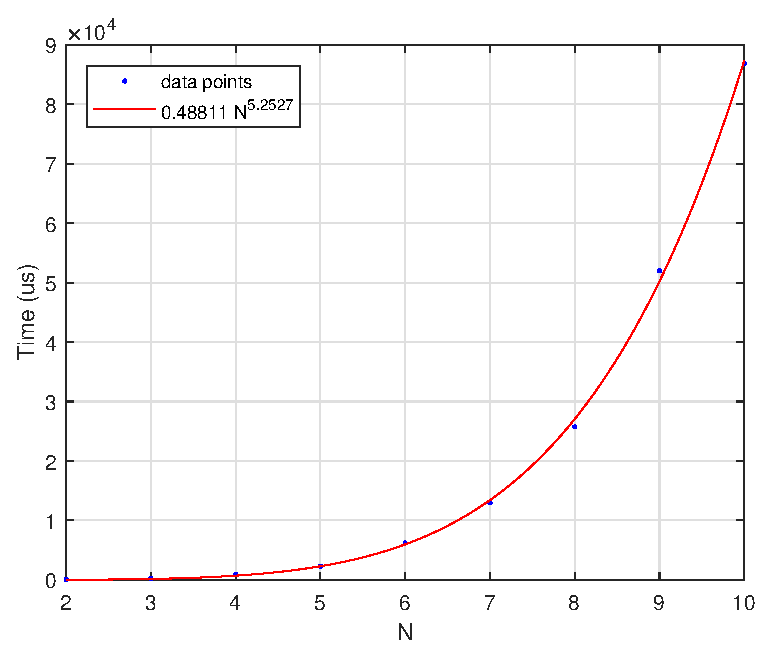
\includegraphics[width=0.6\columnwidth]{question-2/standard_time.eps}
  \caption{Time vs. $N$ for solving the $N * 2N$ mesh of $\SI{1}{\kilo\ohm}$ resistors with the standard circuit solver.}
  \label{fig:q2-std-time}
\end{figure}

We then modified the program to compute and use the half-bandwidth of the matrix $A$ in solving for the Cholesky decomposition. These changes are shown in \Cref{sec:cholesky,sec:solver,sec:circuit-solver-h,sec:circuit-solver-cpp}. Since a node connects only to nodes a distance $N$ away using our numbering system, the half-bandwidth is $b = O(N)$. Hence, the time taken should increase as $O(n b^2)  = O(N^4)$. However, since the initial matrix multiplication $A Y A^T$ is $O(N^6)$, the effects will not be noticeable unless we exclude the time taken to form the initial matrices. To get a better measurement, we measured for $N$ up to $32$. The results are shown in \Cref{fig:q2-band-time}. We fitted a polynomial of the form $a * N ^ b$ to the data and found that it grows approximately as $O(N^4)$. This agrees with the expectation.

\begin{figure}[!htb]
  \centering
  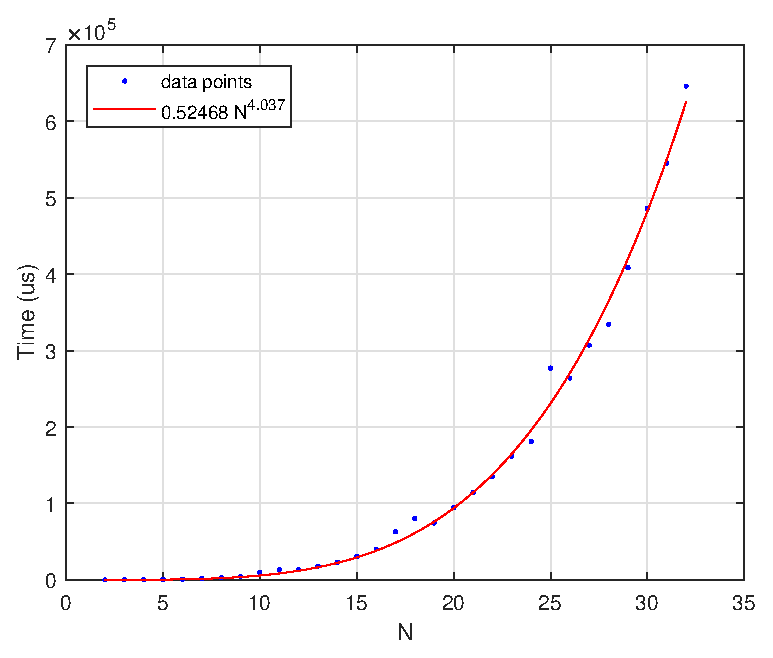
\includegraphics[width=0.6\columnwidth]{question-2/banded_time.eps}
  \caption{Time vs. $N$ for solving the $N * 2N$ mesh of $\SI{1}{\kilo\ohm}$ resistors with the banded circuit solver.}
  \label{fig:q2-band-time}
\end{figure}

We then measured the values of $R$ for $N$ up to $32$ and plotted the results in \Cref{fig:q2-resistance}. After trying different functions to fit the data, we found that the resistance is best approximated by a function of the form $R(N) = a * log(N + b) + c$. The best such function is included in \Cref{fig:q2-resistance}. We can see that this function is an almost perfect fit over the entire range. Thus, we can conclude that, asymptotically, we have $R(N) = O(log(N))$.

\begin{figure}[!htb]
  \centering
  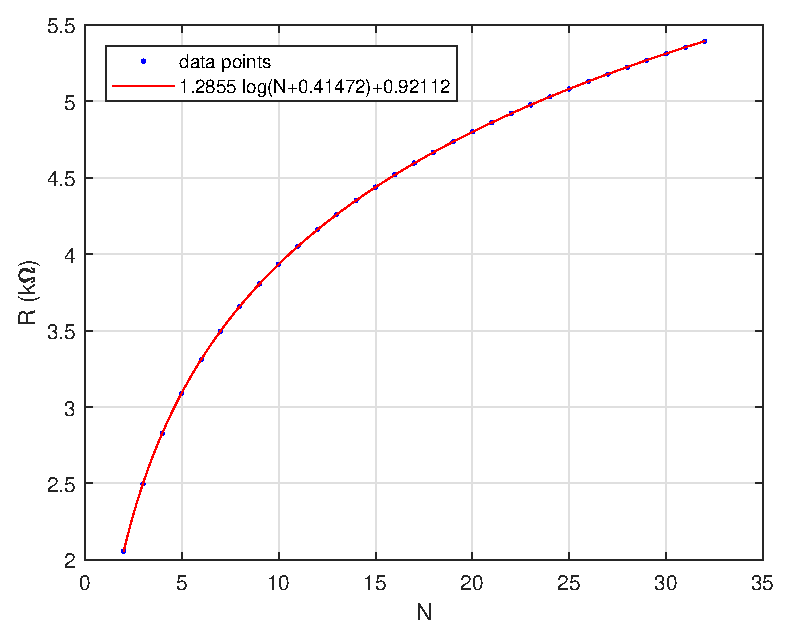
\includegraphics[width=0.6\columnwidth]{question-2/resistance.eps}
  \caption{$R$ vs. $N$ for the $N * 2N$ mesh of $\SI{1}{\kilo\ohm}$ resistors.}
  \label{fig:q2-resistance}
\end{figure}

\section*{Question 3}

We then wrote a program to use a SOR finite difference method to solve for the potential between two conductors, as given in the assignment specifications. We exploited both the vertical and horizontal symmetries to work with only a quarter of the grid. The code is shown in \Cref{sec:main,sec:finite-differences-h,sec:finite-differences-cpp}.

We then set $h = 0.02$ and varied $w$ over the range $[1.0, 2.0)$ in $0.1$ increments. The results are shown in \Cref{tab:q3-w-sor}. The number of iterations taken for each value of $w$ is also plotted in \Cref{fig:q3-w}. We omit the point at $w = 1.9$ to better visualize the data. From this we can see that the value of $w = 1.4$ results in the fastest convergence.

\begin{table}[!htb]
  \centering
  \caption{Results for SOR with $h = 0.02$ for different values of $w$.}
  \label{tab:q3-w-sor}
  \resizebox{0.7\columnwidth}{!}{\begin{tabular}{|l|l|l|}
    \hline
    $w$ & Iterations & $V_{(0.06,0.04)} (\SI{}{\volt})$ \\ \hline
    1.0 & 38 & 5.52627 \\ \hline
    1.1 & 31 & 5.52627 \\ \hline
    1.2 & 26 & 5.52630 \\ \hline
    1.3 & 21 & 5.52631 \\ \hline
    1.4 & 20 & 5.52634 \\ \hline
    1.5 & 25 & 5.52635 \\ \hline
    1.6 & 37 & 5.52634 \\ \hline
    1.7 & 54 & 5.52634 \\ \hline
    1.8 & 92 & 5.52635 \\ \hline
    1.9 & 903 & 5.52632 \\ \hline
  \end{tabular}}
\end{table}

\begin{figure}[!htb]
  \centering
  \includegraphics[width=0.6\columnwidth]{question-3/w_sor.eps}
  \caption{Iterations vs. $w$ for SOR with $h = 0.02$.}
  \label{fig:q3-w}
\end{figure}

We then set $w = 1.4$ and varied $h$. The results are shown in \Cref{tab:q3-h-sor} and plotted in \Cref{fig:q3-h-v-sor,fig:q3-h-iter-sor}. From this data, it is clear that the potential at the point $(0.06, 0.04)$ is dropping as we decrease $h$. However, it is hard to predict what the value is without trying lower values of $h$, which would take too much time. We can estimate that it is between $\SI{5.10}{\volt}$ and $\SI{5.20}{\volt}$. To three significant figures, we could therefore estimate it to be around $\SI{5.14}{\volt}$, but this estimate is very likely to be wrong. We can also observe from \Cref{fig:q3-h-iter-sor} that the number of iterations increases at supra-linear rates. That is, the iterations needed increase faster than $1/h$. This has the consequence that decreasing $h$ to find better approximations rapidly becomes impractical.

\begin{table}[!htb]
  \centering
  \caption{Results for SOR with $w = 1.4$ for different values of $h$.}
  \label{tab:q3-h-sor}
  \resizebox{0.7\columnwidth}{!}{\begin{tabular}{|l|l|l|}
    \hline
    $1/h$ & iterations & $V_{(0.06,0.04)} (\SI{}{\volt})$ \\ \hline
    50 & 20 & 5.52634 \\ \hline
    100 & 62 & 5.35057 \\ \hline
    200 & 209 & 5.28872 \\ \hline
    250 & 308 & 5.27838 \\ \hline
    500 & 1009 & 5.25778 \\ \hline
    1000 & 3215 & 5.23656 \\ \hline
  \end{tabular}}
\end{table}

\begin{figure}[!htb]
  \centering
  \includegraphics[width=0.6\columnwidth]{question-3/h_v_sor.eps}
  \caption{$V_{(0.06,0.04)}$ vs. $1/h$ for SOR with $w = 1.4$.}
  \label{fig:q3-h-v-sor}
\end{figure}

\begin{figure}[!htb]
  \centering
  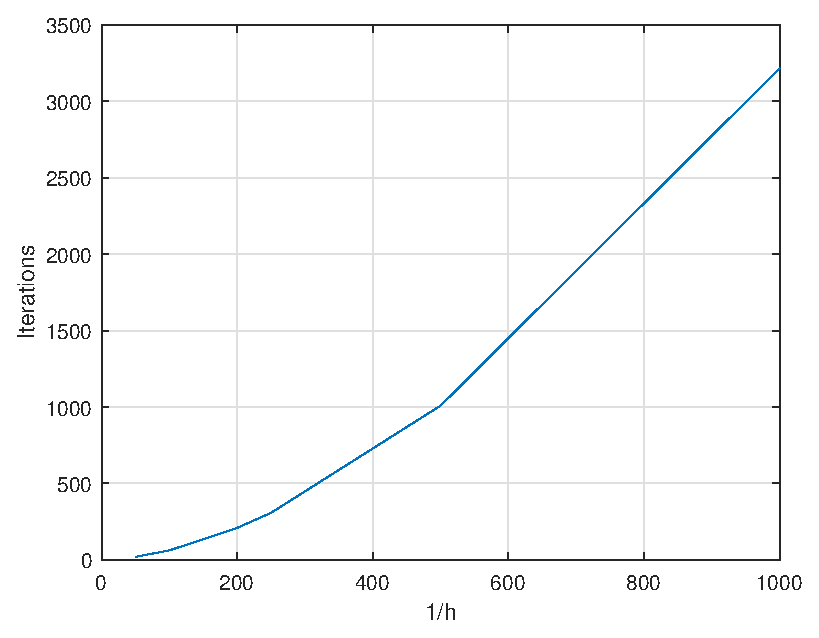
\includegraphics[width=0.6\columnwidth]{question-3/h_iter_sor.eps}
  \caption{Iterations vs. $1/h$ for SOR with $w = 1.4$.}
  \label{fig:q3-h-iter-sor}
\end{figure}

Then, we used the Jacobi method to solve the same problem. The results are shown in \Cref{tab:q3-h-jacobi} and plotted in \Cref{fig:q3-h-v-jacobi,fig:q3-h-iter-jacobi}. From this data, we can see that the Jacobi method requires more iterations than SOR for the same values of $h$. However, the rate of increase appears to be similar. Thus, we conclude that the SOR approach has an initial speed advantage, but as $h$ gets smaller its performance drops at the same rate as the Jacobi method. It is possible that varying the value of $w$ can improve the performance of SOR at these smaller spacings. In addition, we notice that the Jacobi method is more accurate than SOR for the same values of $h$, since the potential it computes is slightly lower.

\begin{table}[!htb]
  \centering
  \caption{Results for the Jacobi method for different values of $h$.}
  \label{tab:q3-h-jacobi}
  \resizebox{0.7\columnwidth}{!}{\begin{tabular}{|l|l|l|}
    \hline
    $1/h$ & iterations & $V_{(0.06,0.04)} (\SI{}{\volt})$ \\ \hline
    50 & 63 & 5.52614 \\ \hline
    100 & 227 & 5.34994 \\ \hline
    200 & 781 & 5.28654 \\ \hline
    250 & 1153 & 5.27505 \\ \hline
    500 & 3764 & 5.24523 \\ \hline
    1000 & 11692 & 5.18932 \\ \hline
  \end{tabular}}
\end{table}

\begin{figure}[!htb]
  \centering
  \includegraphics[width=0.6\columnwidth]{question-3/h_v_jacobi.eps}
  \caption{$V_{(0.06,0.04)}$ vs. $1/h$ for the Jacobi method.}
  \label{fig:q3-h-v-jacobi}
\end{figure}

\begin{figure}[!htb]
  \centering
  \includegraphics[width=0.6\columnwidth]{question-3/h_iter_jacobi.eps}
  \caption{Iterations vs. $1/h$ for the Jacobi method.}
  \label{fig:q3-h-iter-jacobi}
\end{figure}

We then modified the program to allow uneven spacing. An interface was provided where the user could input a vector of $x$ positions and a vector of $y$ positions indicating where grid lines would be located. The code is shown in \Cref{sec:finite-differences-h,sec:finite-differences-cpp}. Using this setup, we separated the grid using the same number of nodes as for $h = 0.01$. We approached this by starting with the grid for $h = 0.02$ and adding lines close to the point $(0.06, 0.04)$ until we got a better result. The resulting $x$ vector was (0.0, 0.02, 0.04, 0.05, 0.055, 0.06, 0.065, 0.07, 0.08, 0.1) and the resulting $y$ vector was (0.0, 0.02, 0.03, 0.04, 0.041, 0.042, 0.045, 0.05, 0.06, 0.07, 0.08, 0.1). Using this setup, we were able to obtain a value of $V_{(0.06,0.04)} = \SI{5.33519}{\volt}$, which is closer to the real value than the value obtained with $h = 0.01$.

% \section{Conclusions}


\newpage
\onecolumn

\begin{appendices}

\section{Main.cpp}
\label{sec:main}
\lstinputlisting[language=C++]{src/main.cpp}
\newpage

\section{Matrix.h}
\label{sec:matrix}
\lstinputlisting[language=C++]{src/matrix.h}
\newpage

\section{Matrix-util.h}
\label{sec:matrix-util}
\lstinputlisting[language=C++]{src/matrix-util.h}
\newpage

\section{Cholesky.h}
\label{sec:cholesky}
\lstinputlisting[language=C++]{src/cholesky.h}
\newpage

\section{Solver.h}
\label{sec:solver}
\lstinputlisting[language=C++]{src/solver.h}
\newpage

\section{Mesh.h}
\label{sec:mesh-h}
\lstinputlisting[language=C++]{src/mesh.h}
\newpage

\section{Mesh.cpp}
\label{sec:mesh-cpp}
\lstinputlisting[language=C++]{src/mesh.cpp}
\newpage

\section{Circuit-solver.h}
\label{sec:circuit-solver-h}
\lstinputlisting[language=C++]{src/circuit-solver.h}
\newpage

\section{Circuit-solver.cpp}
\label{sec:circuit-solver-cpp}
\lstinputlisting[language=C++]{src/circuit-solver.cpp}
\newpage

\section{Finite-differences.h}
\label{sec:finite-differences-h}
\lstinputlisting[language=C++]{src/finite-differences.h}
\newpage

\section{Finite-differences.cpp}
\label{sec:finite-differences-cpp}
\lstinputlisting[language=C++]{src/finite-differences.cpp}
\newpage

\section{Extract from Solver-test.cpp}
\label{sec:solver-test-cpp}
\begin{lstlisting}[language=C++]
TEST_CASE("solve succeeds for a 2x2 system of equations")
{
    Matrix<double> lower = "["
                           "1,0;"
                           "2,1"
                           "]";
    Matrix<double> m = lower * transpose(lower);
    Matrix<double> x = "[4;3]";
    Matrix<double> b = m * x;
    auto result = solve(m, b);
    REQUIRE(result == x);
}

TEST_CASE("solve succeeds for a 3x3 system of equations")
{
    Matrix<double> lower = "["
                           "4, 0,0;"
                           "5, 1,0;"
                           "9,-1,2"
                           "]";
    Matrix<double> m = lower * transpose(lower);
    Matrix<double> x = "[1.0;2.5;-2.0]";
    Matrix<double> b = m * x;
    auto result = solve(m, b);
    REQUIRE(result == x);
}

TEST_CASE("solve succeeds for a 4x4 system of equations")
{
    Matrix<double> lower = "["
                           " 1, 0, 0, 0;"
                           " 2, 3, 0, 0;"
                           " 5, 7,11, 0;"
                           "13,17,19,23"
                           "]";
    Matrix<double> m = lower * transpose(lower);
    Matrix<double> x = "[1;2;4;8]";
    Matrix<double> b = m * x;
    auto result = solve(m, b);
    REQUIRE(result == x);
}

TEST_CASE("solve succeeds for a 5x5 system of equations")
{
    Matrix<double> lower = "["
                           " 1,0,0,0,0;"
                           " 2,1,0,0,0;"
                           " 4,2,1,0,0;"
                           " 8,4,2,1,0;"
                           "16,8,4,2,1"
                           "]";
    Matrix<double> m = lower * transpose(lower);
    Matrix<double> x = "[13;-7;19;-11;3]";
    Matrix<double> b = m * x;
    auto result = solve(m, b);
    REQUIRE(result == x);
}
\end{lstlisting}
\newpage

\section{Extract from Circuit-solver-test.cpp}
\label{sec:circuit-solver-test-cpp}
\begin{lstlisting}[language=C++]
// Truncates the least significant bits of the value for a better floating point
// comparison that ignores some round-off error.
float fround(double value)
{
    return static_cast<float>(value);
}

TEST_CASE("csolve succeeds for circuit 1")
{
    std::stringstream in{"1 0 0 10 0\n"
                         "1 0 0 10 10\n"};
    auto v = csolve(in);
    CHECK(fround(v(0)) == 5.0f);
}

TEST_CASE("csolve succeeds for circuit 2")
{
    std::stringstream in{"1 0 10 10 0\n"
                         "1 0 0 10 0\n"};
    auto v = csolve(in);
    CHECK(fround(v(0)) == 50.0f);
}

TEST_CASE("csolve succeeds for circuit 3")
{
    std::stringstream in{"1 0 0 10 10\n"
                         "1 0 10 10 0\n"};
    auto v = csolve(in);
    CHECK(fround(v(0)) == 55.0f);
}

TEST_CASE("csolve succeeds for circuit 4")
{
    std::stringstream in{"1 0 0 10 10\n"
                         "1 0 0 10 0\n"
                         "1 2 0 5 0\n"
                         "2 0 10 5 0\n"};
    auto v = csolve(in);
    CHECK(fround(v(0)) == 20.0f);
    CHECK(fround(v(1)) == 35.0f);
}

TEST_CASE("csolve succeeds for circuit 5")
{
    std::stringstream in{"1 0 0 20 10\n"
                         "1 2 0 10 0\n"
                         "1 3 0 10 0\n"
                         "2 3 0 30 0\n"
                         "2 0 0 30 0\n"
                         "3 0 0 30 0\n"};
    auto v = csolve(in);
    CHECK(fround(v(0)) == 5.0f);
    CHECK(fround(v(1)) == 3.75f);
    CHECK(fround(v(2)) == 3.75f);
}
\end{lstlisting}

\end{appendices}

\end{document}
